%!TEX root = ../Thesis.tex

\chapter{Detecting the board}
	\label{detector}
	When looking at a Go board what first catches one's eye are the lines. As we said before, though, relying solely on lines for the detection of the grid will probably fail in endgame situations. Therefore our algorithm uses them only to find intersections and tries to fill in gaps by adding information about pieces, too. This was born out of the idea that what is actually interesting are not the lines, but their intersections and a piece will always lie reasonably close to one. We also rely on the user placing the camera or the board such that the center of the board is located in the center of the screen.

	Our implementation was based on the OpenCV framework in its current version 2.4.10 and where not noted otherwise all detection has been performed on x86\_64 architecture. As described in chapter 3 this does not seem to provide different results than execution on mobile devices (i.e. ARM architecture), for example because of differences in floating point calculations.

	In short we do the following steps:
	\begin{enumerate}
		\item roughly pre-segment the board by analyzing connected components around the center of the thresholded input image
		\item detect horizontal and vertical lines and intersect them
		\item detect pieces on the board and consider their centers intersections, too
		\item remove duplicates
		\item select a few intersections around the center of the image
		\item build a submodel of the board by estimating where each selected point lies on the grid
		\item calculate their position in space using RANSAC and applying the resulting transformation matrix to a complete model of the board
	\end{enumerate}

	\section{Preprocessing}
	\label{detector-preprocessing}
	Mobile devices don't have the same computing power as desktop hardware does. Therefore our first step is to reduce the image size without losing relevant information. To do so, we threshold the grayscale input image using a mean adaptive threshold with a low constant value \emph{C} and a window size of what we expected to be roughly the width of one square on the board (approximately 45px, as measured in one of our sample images).

	Under the assumption that at least part of the board is in the center of the image we can segment it now from the background with high confidence by a simple connect-component analysis. On our test case this fails only in one situation where the board lies in grass in the evening. Hard shadows connect the board with the background. On a flat surface this is not a problem.

	This step does not just improve speed but also detection performance because interfering background information like patterned wood table tops can be cut off.

	\section{Detecting visible intersections}
	\subsection{Using Hough lines detection}
	\label{detector-visible-hough}
	Having cropped the image to the board we use line detection to find the visible grid lines. For this we evaluated two different well known methods. Our first approach was to use probabilistic hough lines after applying a Canny edge detector. We furthermore found, that blurring the image with a light Gaussian improves detection quality and speed.

	For each line the absolute pitch to the x-axis and the y-axis of the image is calculated and compared to a specific threshold. Initially we set this pretty high to eliminate as many false lines as possible from the image, however it turned out that the image segmentation in the first step allows us to lower the value to one, i.e. each line is either classified as horizontal or vertical and only perfectly diagonal lines are discarded.

	The resulting lines can now be intersected with each other. We are using the whole line, not just line segments here, because then it is sufficient to detect a short part of a grid line.

	\subsection{Using LSD}
	\label{detector-visible-lsd}
	%TODO update with  updated algorithm
	We then tried applying the Line Segment Detector \cite{von2012lsd} on the output of the Canny edge detector. We had to backport this from OpenCV 3 as it is not available in the aforementioned version. Surprisingly it turned out to be too exact and requires significant post-processing. For every square in the grid the LSD finds four line segments. Consequently two adjacent squares produce two parallel lines. This method is also very prone to noise and produces many short, false positive lines, especially around game pieces, as can be seen in \ref{fig:lsdPostprocessingFirst}.

	Therefore our first postprocessing step is to eliminate short line segments (see \ref{fig:lsdPostprocessingLength}). Afterwards for each line we count the number of parallels close-by and keep only those with a count of at least one, as most line segments pertaining to the grid have a parallel line. Having reduced the number of false positives significantly we classify the lines the same way as described above into horizontal and vertical lines. If we now intersected those, we would still have many false positives, because one line which spans the whole length of the grid on the board might be represented by several detected line segments. As we prolong them into infinity when intersecting small differences in direction add up and produce intersections at the wrong place. Thus as last postprocessing step we merge nearby line segments into one if they are close and parallel to each other and filter once again for line length, this time with a slightly higher threshold.

	\begin{figure}
		\begin{subfigure}{0.23\textwidth}
			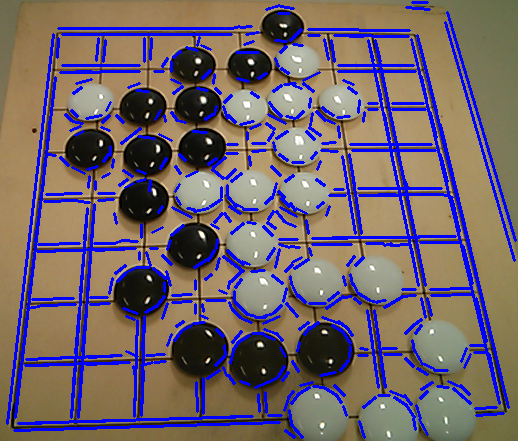
\includegraphics[width=\textwidth]{images/lsd_first.png}
			\label{fig:lsdPostprocessingFirst}
			\caption{Unfiltered LSD output}
		\end{subfigure}
		\hfill
		\begin{subfigure}{0.23\textwidth}
			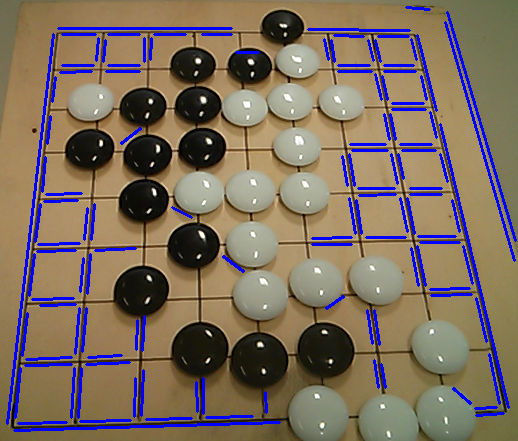
\includegraphics[width=\textwidth]{images/lsd_length.png}
			\label{fig:lsdPostprocessingLength}
			\caption{... filtered for line length,}
		\end{subfigure}
		\hfill
		\begin{subfigure}{0.23\textwidth}
			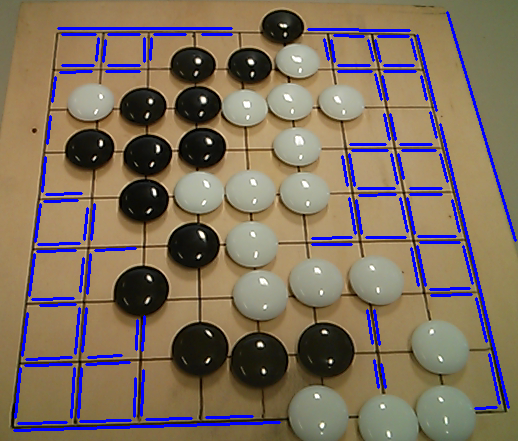
\includegraphics[width=\textwidth]{images/lsd_parallel.png}
			\label{fig:lsdPostprocessingParallel}
			\caption{... filtered for parallels, }
		\end{subfigure}
		\hfill
		\begin{subfigure}{0.23\textwidth}
			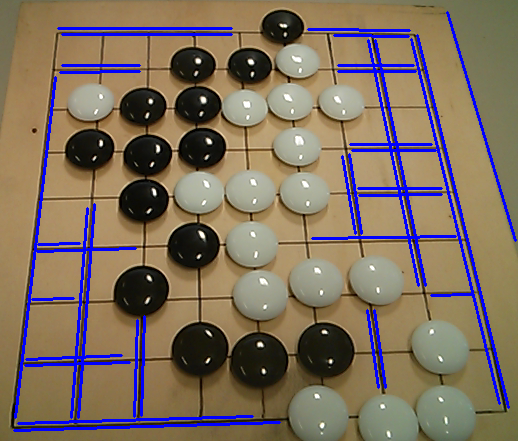
\includegraphics[width=\textwidth]{images/lsd_final.png}
			\label{fig:lsdPostprocessingFinal}
			\caption{and stitched and filtered for length}
		\end{subfigure}

		\caption{The postprocessing steps necessary for the LSD}
	\end{figure}


	\subsection{Using corner detectors}
	\label{detector-visible-corners}
	Another option to detect the intersection directly without line detection might be to use a corner detector. We tested the FAST \cite{rosten2006machine} detector on a slightly blurred image for this task. However it provides too many false positives to be of any use. Especially around black stones it is extremely unreliable. The ORB detector which uses FAST internally does not increase quality either.

	\section{Detecting occluded intersections}
	\subsection{Using Hough circles}
	\label{detector-occluded-hough}
	Go pieces are relatively round and can be detected using Hough circles to some extent. Applying the algorithm to the output of a Canny edge detector on the original grayscale image failed, though. The reason lies with the squares of the board and the images being taken from an angle. In order to still match the pieces the threshold in the accumulator space beyond which a circle center will be detected has to be chosen quite low. This results in many false positives at the center of the squares.

	To remove the lines and have only the pieces themselves remaining we tried thresholding the image. This works quite well for the black pieces. The white pieces on the other hand cannot be reliably detected this way. This is because the contrast between white pieces and the board is too low. We therefore turned to color images. We convert those from OpenCV's native BGR into HSV color space and threshold the value channel for black pieces, again with good results.

	%TODO: die zwei klammern neu formulieren, das ist ja grausam. am besten ganzen absatz.
	White pieces cannot be detected in the value channel because the contrast there is too low. In the other channels they remain hard to detect, too, as the white balance of the camera input is constantly being adjusted by the operating system. This leads to color aberrations when a player puts down a stone and his or her hand takes up lots of the image: the image will change its color temperature and white pieces become slightly blue. Often the aberration will be corrected after the hand leaves the image, but depending on the background this does not happen every time. Luckily the white pieces are well detectable under normal circumstances in the saturation channel (saturation of the pieces is low and of the board is high, hue is undefined) and when the color is shifted in the hue channel (saturation of the pieces and the board is low, hue of the pieces is low).

	Therefore we threshold the saturation and the hue channel separately, count the non-zero responses and use the individual results only if at most 20\% of the image is below the threshold.

	This yields pretty good results, however there is still a lot of noise in the thresholded image. To reduce this we apply a Gaussian blur to the source image before thresholding and remove speckles afterwards by eroding and dilating the image slightly.

	Even still black pieces are being detected better, as we describe in chapter five. However it is not very important to us to have a perfect detection ratio in this step, because the results are not used to generate the end result but only to fill in gaps in the intersections previously detected.

	The centers of the detected circles are then added to intersections and duplicates (determined by their distance) are removed.

	\subsection{Using contours}
	\label{detector-occluded-contours}
	Finding pieces with hough transformation is slow, though, and we were not contempt with the result to speed ratio. That is why we investigated further and chose to try analyzing the image topologically using OpenCV's \emph{findContours} function.

	We preprocess the image the same way as before. This results in blobs for each piece whose contours can be detected nicely. Those can then be fitted nicely into quadratic rectangles. All contours whose bounding box is not more or less quadratic we discard. Sometimes two stones next to each other meld into one blob and result in non-quadratic bounding boxes. Those could be split into two, but we did not see the need for that.

	The centers of the detected squares are then added to intersections just like the centers of the circles when using hough transformation.

	\section{Calculating missing intersections}
	\label{detector-calculate}
	Having collected a set of probable intersections we now must fill in gaps where neither lines nor pieces have been detected. Also we need to somehow figure out which detected intersections are valid and actually are part of the board and which are simply intersections of grid lines with the outer edge of the board or other noise.

	First we calculate the average angle of the horizontal lines from the previous step and rotate the image to justify them. Then we select a number of intersections in the center of the board by selecting all intersections inside a square around the center. To do so, we assume the center of the board is the closest (detected or yet undetected) intersection to the center of the image. While this assumption can hardly be made in setups where the image is taken by bystanders or from randomly located cameras, we argue that when trying to record a game a user will be able to adjust the camera location accordingly. Another possibility could be to prompt the user for the center of the board, which is easily done via the touchscreen of the smart phone. We did not implement this approach for time reasons, but it should yield equal quality.

	%TODO: anzahl evaluieren und hier eintragen
	If the number of selected intersections is too small, we increase the window size and try again.

	Those intersections are now modeled as a subset of actual board intersections. We determine the median distance between neighboring intersections -- using the mean yielded worse results. Then we iterate row-wise over the selected intersections from the top left to the bottom right (to facilitate this we sort the intersections before selection). For every intersection we save the current row and column (on the board, not the image) and add a key point to our model at this location. If we encounter a gap between two intersection that is larger than the median distance we increase the column count accordingly. The same happens in y-direction with the row count. If we find an intersection is an outlier to the left we increase the column count of all previous key points accordingly.

	The interim result of this iteration is a submodel of the board with equidistant key points where every key point correspondents to a selected intersection.

	During the iteration we also add virtual intersections to fill in gaps in our intersection set. From this filled up intersection set we select the intersection closest to the image center and assume it is the intersection in the center of the board. Using the center intersection row and column count we can shift our model to the correct position within the board.

	Our updated interim result is now a submodel of the board located correctly inside the whole model, which we can feed into the RANSAC algorithm, as we made sure every key point corresponds to an intersection thus creating homography between them. This serves three purposes. First, the RANSAC algorithm tolerates outliers, i.e. intersections which have been detected slightly wrong. Second, we can use the homography information to rectify subsequent images and increase detection quality. Lastly the transformation matrix can also be used to warp a complete model of the board and lay it onto the image. Now we know the location of every intersection -- including those, which have not been detected previously.

	\section{Postprocessing}
	\label{detector-postprocessing}

	\section{Classifying intersections}
	\label{detector-classifying}
	We can now evaluate the board at the intersections to find whether there's a piece there or not and if so of which color it is. The first step here is to use an adaptive threshold and to segment the board using a connect component analysis similarly to the preprocessing step. The result is a binary image showing only the lines and black pieces. Highlights within the black pieces from reflections are still a problem but can be removed well enough by erosion and dilution.

	For every intersection we calculate the average pixel value in a window and compare it to two thresholds, such that \begin{equation}
		\frac{\sum^{I,J}_{i=0,j=0}w(i,j)}{I*J} =
		\begin{cases}
		> T_{w} + C & \Rightarrow  \text{white}\\
		< T_{b} & \Rightarrow \text{black}\\
		\text{otherwise} & \Rightarrow \text{empty}
		\end{cases}
	\end{equation}
	where $C$ is a constant value that is added to the white threshold on the edge of the grid. This is necessary because the lines are not continued there and less black pixels from them are contributed.

	%TODO: evtl postprocessing (gleitender durchschnitt der intersections)
	%TODO: rotation der intersections
	%TODO: unsegmentation der intersections
